\documentclass[11pt]{article}
\usepackage[margin=1in]{geometry}
\usepackage{lmodern}
\usepackage[T1]{fontenc}
\usepackage{titlesec}
\usepackage{titling}
\usepackage{hyperref}
\usepackage{enumitem}
\usepackage{graphicx}
\usepackage{tikz}
\usetikzlibrary{shapes, arrows, positioning, calc}

\hypersetup{
    colorlinks=true,
    linkcolor=blue,
    urlcolor=blue,
    pdftitle={PromptScript Technical Whitepaper},
    pdfauthor={Leomuguchia}
}

\title{PromptScript Technical Whitepaper}
\author{Leomuguchia}
\date{\today}

% Section formatting
\titleformat{\section}{\Large\bfseries}{\thesection.}{1em}{}
\titleformat{\subsection}{\large\bfseries}{\thesubsection.}{1em}{}
\titleformat{\subsubsection}{\normalsize\bfseries}{\thesubsubsection.}{1em}{}

\begin{document}

\maketitle
\tableofcontents
\newpage

\section{Introduction}

\subsection{Motivation}
PromptScript is an open source DSL and AI orchestration platform that converts high-level developer intents into executable code. Leveraging modern AI language models and a structured prompt engineering approach, PromptScript aims to:
\begin{itemize}[leftmargin=1.5em]
    \item \textbf{Reduce the barrier to coding:} Enable non-experts to describe functionality in a semi-structured format.
    \item \textbf{Accelerate prototyping:} Rapidly convert ideas into runnable code.
    \item \textbf{Unify human intent and machine execution:} Create a consistent workflow from ideation to deployment.
\end{itemize}

\subsection{Scope}
This document outlines the technical design of PromptScript, focusing on:
\begin{itemize}[leftmargin=1.5em]
    \item DSL syntax and structure.
    \item Context management and multi-step reasoning.
    \item AI orchestration and code generation pipeline.
    \item Integration with deployment workflows.
\end{itemize}

\section{System Architecture}

\subsection{High-Level Architecture Diagram}
\begin{center}
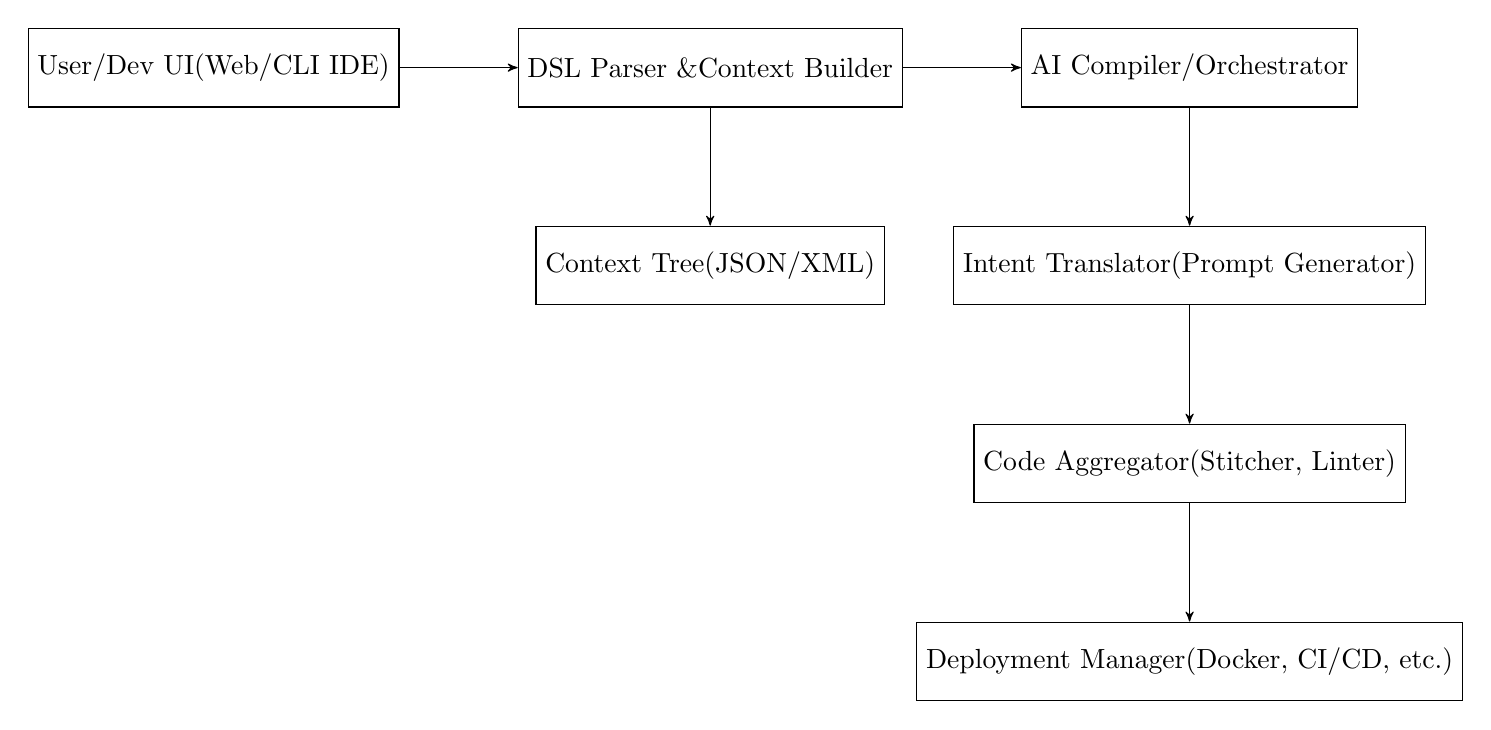
\begin{tikzpicture}[node distance=1.5cm, auto, >=stealth']
    % Nodes
    \node (ui) [draw, rectangle, text centered, minimum width=3cm, minimum height=1cm] {User/Dev UI\\(Web/CLI IDE)};
    \node (parser) [draw, rectangle, right=of ui, text centered, minimum width=3cm, minimum height=1cm] {DSL Parser \&\\Context Builder};
    \node (compiler) [draw, rectangle, right=of parser, text centered, minimum width=3cm, minimum height=1cm] {AI Compiler/\\Orchestrator};
    \node (contextTree) [draw, rectangle, below=of parser, text centered, minimum width=3cm, minimum height=1cm] {Context Tree\\(JSON/XML)};
    \node (translator) [draw, rectangle, below=of compiler, text centered, minimum width=3cm, minimum height=1cm] {Intent Translator\\(Prompt Generator)};
    \node (aggregator) [draw, rectangle, below=of translator, text centered, minimum width=3cm, minimum height=1cm] {Code Aggregator\\(Stitcher, Linter)};
    \node (deploy) [draw, rectangle, below=of aggregator, text centered, minimum width=3cm, minimum height=1cm] {Deployment Manager\\(Docker, CI/CD, etc.)};
    
    % Arrows
    \draw[->] (ui) -- (parser);
    \draw[->] (parser) -- (compiler);
    \draw[->] (parser) -- (contextTree);
    \draw[->] (compiler) -- (translator);
    \draw[->] (translator) -- (aggregator);
    \draw[->] (aggregator) -- (deploy);
\end{tikzpicture}
\end{center}

\subsection{Component Overview}
\begin{description}[leftmargin=1.5cm]
    \item[User Interface (UI):] Web-based or CLI editor for authoring PromptScript. Provides real-time display of parsed context and generated code fragments.
    \item[DSL Parser \& Context Builder:] 
    \begin{itemize}
        \item \textbf{Parser Engine:} Built using Python (or tools like ANTLR) to tokenize and parse PromptScript.
        \item \textbf{Context Builder:} Organizes parsed tokens into a hierarchical context tree (global project settings, prompt blocks, workflows).
    \end{itemize}
    \item[Intent Translator:] Converts DSL blocks into structured AI prompts. Uses chain-of-thought techniques for multi-step reasoning and context augmentation.
    \item[AI Compiler/Orchestrator:]
    \begin{itemize}
        \item \textbf{AI Query Executor:} Connects to AI language models (e.g., OpenAI’s GPT-4) to generate code.
        \item \textbf{Session Context Manager:} Maintains state and passes global/local context between queries.
        \item \textbf{Meta-Prompter:} Monitors responses for consistency and re-prompts if needed.
    \end{itemize}
    \item[Code Aggregator:] Combines generated code fragments into a cohesive codebase. Ensures dependency resolution and integrates formatting/linting tools.
    \item[Deployment Manager:] Provides containerization (Docker support) and integrates with cloud providers (e.g., Kubernetes, AWS). Automates build, test, and deployment via CI/CD pipelines.
\end{description}

\section{Detailed Component Specifications}

\subsection{DSL Parser \& Context Builder}

\subsubsection{DSL Syntax Overview}
A sample PromptScript snippet:
\begin{verbatim}
blueprint ToDoApp {
    version: "1.0"
    author: "ChatGPT"
    goal: "Develop a full-stack to-do app with user authentication, task management, and dynamic UI."
}

prompt UserAuth {
    define Data:
        User { email: string, password: string, verified: bool }
    
    task register:
        input: User user
        instruction: "Store user data securely and send a verification email."
        output: "registrationStatus"
    
    task login:
        input: email: string, password: string
        instruction: "Authenticate the user and generate a session token."
        output: "sessionToken"
}

workflow ToDoFlow {
    step auth -> UserAuth.login(email, password)
    step addTask -> TaskManager.create(title)
}
\end{verbatim}

\subsubsection{Parser Implementation}
\begin{itemize}
    \item \textbf{Language:} Python 3.x  
    \item \textbf{Parsing Technique:} 
    \begin{itemize}
        \item Use regular expressions for a proof-of-concept.
        \item Future iterations may leverage parser generators (e.g., ANTLR) for robustness.
    \end{itemize}
    \item \textbf{Output Data Structure:} The parser produces a JSON-like context tree:
\begin{verbatim}
{
    "blueprint": {
        "name": "ToDoApp",
        "properties": {
            "version": "1.0",
            "author": "ChatGPT",
            "goal": "Develop a full-stack to-do app..."
        }
    },
    "prompts": [
        {
            "name": "UserAuth",
            "tasks": [
                {
                    "name": "register",
                    "input": "User user",
                    "instruction": "Store user data securely...",
                    "output": "registrationStatus"
                },
                {
                    "name": "login",
                    "input": "email: string, password: string",
                    "instruction": "Authenticate the user...",
                    "output": "sessionToken"
                }
            ]
        }
    ],
    "workflow": {
        "name": "ToDoFlow",
        "steps": [
            "UserAuth.login(email, password)",
            "TaskManager.create(title)"
        ]
    }
}
\end{verbatim}
\end{itemize}

\subsection{Intent Translator \& AI Compiler}

\subsubsection{Intent Translation}
\begin{itemize}
    \item \textbf{Function:} Transform DSL blocks into AI-friendly prompt strings.
    \item \textbf{Chain-of-Thought Example:} For the task \texttt{UserAuth.login}, the generated prompt might be:
    \begin{quote}
    ``You are an AI developer tasked with generating a Python Flask endpoint. The function should accept JSON with an \texttt{email} and \texttt{password}, authenticate the user, and return a session token. Please include proper error handling and follow secure coding practices.''
    \end{quote}
    \item \textbf{Context Augmentation:} Combines global blueprint details (e.g., app version, architectural stack) with local prompt data.
\end{itemize}

\subsubsection{AI Compiler/Orchestrator}
\begin{itemize}
    \item \textbf{Technology:} Python-based microservice interacting with external AI APIs.
    \item \textbf{Modules:}
    \begin{itemize}
        \item \textbf{Session Context Manager:} Manages conversation state using caching (e.g., Redis) for persistent context.
        \item \textbf{Query Executor:} Assembles prompts and sends them to AI services (using asynchronous calls for speed).
        \item \textbf{Meta-Prompter:} Evaluates responses for consistency and triggers additional prompts if key elements are missing.
    \end{itemize}
    \item \textbf{API Integration:} Uses REST/GraphQL interfaces to communicate with AI platforms, ensuring secure API keys and rate limiting.
\end{itemize}

\subsection{Code Aggregator \& Deployment Manager}

\subsubsection{Code Aggregator}
\begin{itemize}
    \item \textbf{Stitching Engine:} Combines multiple language fragments (e.g., backend code in Python, frontend in JavaScript) into a coherent project structure.
    \item \textbf{Dependency Resolver:} Maps symbols (classes, functions) across modules to ensure inter-dependencies are met.
    \item \textbf{Formatting:} Integrates with linters/formatters (e.g., Black, Prettier, ESLint) to standardize code style.
\end{itemize}

\subsubsection{Deployment Manager}
\begin{itemize}
    \item \textbf{Containerization:} Generates Dockerfiles and Kubernetes YAML configurations.
    \item \textbf{CI/CD Integration:} Provides scripts for platforms like GitHub Actions or Jenkins for automated testing and deployment.
    \item \textbf{Cloud Connectors:} Configurations for deploying to cloud platforms (e.g., AWS Elastic Beanstalk, Google Cloud Run).
\end{itemize}

\section{Context Management \& Reasoning Strategies}

\subsection{Hierarchical Context Tree}
\begin{itemize}
    \item \textbf{Global Context:} Stored in a central JSON file including blueprint details.
    \item \textbf{Local Context:} Each prompt/task node inherits context from its parent.
\end{itemize}

\subsection{Dynamic Context Window Optimization}
\begin{itemize}
    \item \textbf{Summarization:} Use summarization APIs to condense long contexts when token limits are reached.
    \item \textbf{Pinning Critical Data:} Always include blueprint metadata and primary module dependencies in every prompt.
\end{itemize}

\subsection{Multi-Agent Reasoning (Future Work)}
\begin{itemize}
    \item \textbf{Agent Roles:}
    \begin{itemize}
        \item \textbf{Architect Agent:} Plans overall project structure.
        \item \textbf{Coder Agent:} Generates code for individual tasks.
        \item \textbf{Reviewer Agent:} Analyzes and refines generated code.
        \item \textbf{Deployment Agent:} Packages and deploys the final output.
    \end{itemize}
    \item \textbf{Coordination:} Agents share a unified context tree and communicate via internal APIs.
\end{itemize}

\section{Implementation Roadmap}

\subsection{Phase 1: Prototype Development}
\begin{itemize}
    \item Build a minimal parser and context builder.
    \item Create a simple web-based editor (using React or similar).
    \item Implement basic integration with a chosen AI API (e.g., OpenAI).
\end{itemize}

\subsection{Phase 2: MVP}
\begin{itemize}
    \item Extend DSL support for more complex constructs (voice commands, conditional workflows).
    \item Develop the full orchestration engine with session context management.
    \item Build the code aggregator and integrate basic deployment scripts.
\end{itemize}

\subsection{Phase 3: Optimization \& Expansion}
\begin{itemize}
    \item Optimize context window strategies with summarization techniques.
    \item Introduce multi-agent reasoning and collaborative AI modules.
    \item Expand deployment support and CI/CD integration.
    \item Open source the project and build a community around PromptScript.
\end{itemize}

\section{Conclusion}
PromptScript represents a bold step toward unifying human intent and machine-executed code generation. With its structured DSL, robust context management, and deep AI integration, PromptScript has the potential to democratize software development and accelerate innovation. The technical foundation outlined in this document provides a roadmap for developing an AI-driven development ecosystem—from prompt to production.

\section{Call to Action}
We invite contributors, researchers, and developers to join the PromptScript project. Let’s collaborate on building an open source platform that redefines how code is conceived, generated, and deployed in the AI age.

\vspace{1em}
\noindent\textbf{Prepared by:} Leomuguchia \\
\textbf{Date:} \today

\end{document}
